% Chapter Template

\chapter{HRI Design and Evaluation} % Main chapter title

\label{Chapter6} % Change X to a consecutive number; for referencing this chapter elsewhere, use \ref{ChapterX}

\lhead{Chapter 6. \emph{HRI Design and Evaluation}} % Change X to a consecutive number; this is for the header on each page - perhaps a shortened title

\section{HRI Design and Evaluation}
The experience of interacting with a robot has been shown to be very different in comparison to people’s interaction experience with other technologies and artifacts, and often has a strong social or emotional component — a difference that poses potential challenges related to the design and evaluation of HRI. Nevertheless, the evaluation methods used in Human Computer Interaction(HCI) has been used as the starting point in developing those for HRI. 

\subsection{Data collection}
	Data collection is one of the important steps in the evaluation process. There are five key issues in the data gathering\cite{Rogers2011}. They are \emph{Identifying participants}:Decide who to gather data from,\emph{Relationship with participants}: Clear and professional,\emph{Setting goals}: Decide how to analyze data once collected,Informed consent when appropriate,\emph{Triangulation}:Look at data from more than one perspective,\emph{Pilot studies}:Small trial of main study. 

\subsection{Holistic interaction experience:}
Young et al.,\cite{Young2011} propose \emph{holistic interaction experience} and introduce a set of three perspectives.

\begin{itemize}
\item Visceral factors of interaction(P1): It focuses on a person’s biological, visceral, and instinctual involvement
in interaction. This includes such things as instinctual frustration, fear, joy, happiness, and so on, on a reactionary level where they are difficult to control.

\item Social mechanics(P2): It focuses on the higher-level communication and social techniques used in interaction. This includes both the social mechanics that a person uses in communication as well as what they interpret from the robot throughout meaning-building during interaction. Examples range from gestures such as facial expressions and body language, to spoken language, to cultural norms such as personal space and eye-contact rules.

\item Social Structures(P3): It covers the development of and changes in the social relationships and interaction between two entities, perhaps over a relatively long period of time (longer relative to P1 and P2). P3 considers the changes in or trajectory of P1, P2, as well as how a robot interacts with, understands, and even modifies social structures.

\end{itemize}

The three perspectives proposed above are used as concrete tools throughout the evaluation process. For doing so, the evaluation process is broken down into 

\begin{itemize}
\item Study Design: In most cases, the study begins with formalizations of research questions and hypotheses. The perspectives help articulate the social characteristics of interaction experience. Additionally they provide a mechanism by which the experimenter can define the focus of their particular interest. For example, a person may hypothesize that a particular robot will elicit happiness and pleasure (P1: visceral reactions). When this occurs, the person will respond by using some social mechanics (P2), such as smiling broadly or bobbing their head. The perspectives can also be used in the design of the evaluation itself, providing clear mechanisms for directed brainstorming and discussion. In particular, they can help assess if and how the types of questions in the study address the targeted social interactions

\item Conducting the study: While the study is being conducted, the three perspectives can serve as a means to remind the evaluator of various social issues of importance. The three perspectives can be used during task completion and efficiency-type explorations to raise more socially oriented questions, such as how the person’s P1 reactions or the robot’s P2 communication are related to the observations, or how the observed results may influence the broader social structures (P3). The perspectives can also be integrated directly into the data collection instrumentation, e.g. note paper could have pre-generated sections that highlight P1, P2, P3. For physiological measurements the perspectives can help widen or help define the target information of interest to the observer.

\item Analysis of Data and Results: For the analysis of the evaluation results, the three perspectives can be used to dissect and direct data exploration. P1, P2, P3 can be used to keep the experimenter grounded on the participant’s experience and to remain explicitly focused on the social aspects of interaction. expressed. As an example, in a hypothetical study, “People found the robot to be creepy, which they expressed both in P1-type externalized reactions and P2 gestures such as ‘keep away’ hand gestures, and this had very strong P3-type interactions with the home.” In this example, the perspectives highlight the difference between perhaps sometimes involuntary P1 and voluntary P2 interactions, and the more individual P1, P2 in comparison to related P3 social structure impacts, which are perhaps more difficult to describe without the perspectives.

\end{itemize}

\begin{figure}[H]
\centering
\begin{subfigure}[b]{0.4\textwidth}
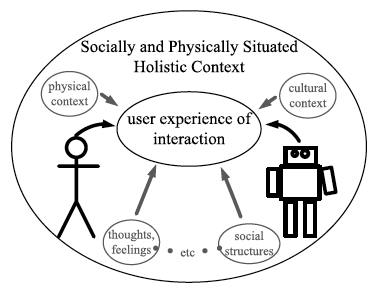
\includegraphics[width=\textwidth]{assets/holistic_view.png}
\caption{A person’s experience of interacting with a robot is influenced
by many real-world social and physical factors, where the robot itself
plays an active role similar to that of a living entity}
\label{fig:holistic_view}
\end{subfigure}%
\hfill
\begin{subfigure}[b]{0.5\textwidth}
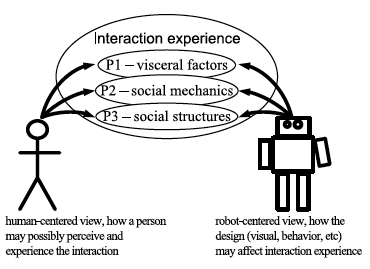
\includegraphics[width=\textwidth]{assets/holistic_interaction_map.png}
\caption{Interaction experience, mutually shaped by two active agents:
human and robots}
\label{fig:holistic_map}
\end{subfigure}%
\caption{Holistic interaction experience}
\label{fig:holistic}
\end{figure}

In addition to proposing three perspective approach, this study also propose an \emph{interaction experience map} which acts as a database of a range of interaction possibilities and outcomes for a particular HRI scenario. The key point is both the human-centered and robot centered views are considered and the three perspectives serve as  brainstorming and sensitizing tools. For the human-centered view, the evaluator can start by brainstorming possible interaction scenarios which may happen in regards to a person and the particular robot or interface. In this stage of the process the evaluator generates a list of high-level scenarios that could conceivably take place, such as, e.g., a person trying to have an extended conversation with the robot even though the robot does not intelligently respond, or the person completely ignoring the robot, and so forth. Then, for each scenario listed in the first step, P1, P2, P3 can be used as probes to consider the interaction experience possibilities within the scenarios, and to sensitize the exploration to the particular social considerations. Simultaneous to the human-oriented exploration, a similar process is followed for the robot-centered case. First, the experimenter brainstorms robot design characteristics that they expect may influence the interaction experience. Then, for each characteristic that was identified, the experimenter considers how people may react to it, and thus, how it may influence interaction experience. Here the three perspectives can be used as exploration probes

\subsection{Social vs Useful HRI}

Baddoura et al.,\cite{Baddoura2013} explore the human affective state of the familiar during a new or unknown situation as it relates to interacting with a robot. In a real unannounced interaction, the measurement of the familiar experienced by two humans interacting with a robot and the intensity and adequacy of their response to its proactive social (greetings) and practical (task to fulfill) actions is performed. An analysis is done on the participants’ reactions to the robot’s actions, the motion of their arms, and their answers to some parts of a questionnaire designed to measure their experience of the familiar and the robot’s sociability. This study aims at learning more about the familiar state in its relation to a satisfying, efficient and reciprocal HRI. The important hypotheses considered are

\begin{itemize}
\item (H1) Experiencing a high level of familiarity when interacting with a robot co-occurs with high levels of adequate responses to its proactive engaging actions (H1/A social actions; and H1/B utilitarian actions).
\item (H2) The change of behavior of the robot from one participant to the other regarding a similar interaction has an effect on the intensity of the familiarity experienced during this interaction as well as on human readiness to interact with the robot afterwards.
\item (H3) The higher the appreciation of the robot’s sociable character is, the more intense is the human response to its engaging actions (H3/A: social actions; and H3/B utilitarian actions).
\item (H4) The more the participants tend to engage in and to react adequately to the robot in a useful joint task initiated by it, the more they tend to respond to the robot’s social solicitations (greeting gestures).
\end{itemize}

The study is conducted with 20 pair of students interacting with the NAO robot on two social tasks and a practical task. The participants are equipped with IMU sensors on their heads and hands in order to measure the intensity of their response during the interaction. Additionally the whole interaction is recorded in order to evaluate the facial response of the participants. The interaction was designed in such a way that the NAO reacts with both the participants in the same way except that it will exhibit a slight hesitation when it interacts with one of the participant. This is intentional in order to measure the effect of change in behavior of the robot during interaction. A questionnaire is also proposed in the native language of the participants addressing different topics. Sometimes same topics are considered from different perspectives. 

The statistical analysis performed during the study showed that (1) the higher the familiar is experienced while interacting with the robot, the more participants responded to its practical action; no similar interdependency was found regarding its social actions; (2) the change of behavior of the robot between participants had no significant effect on the familiar experienced nor on the readiness to respond to the robot; (3) the higher the appreciation of the robot’s sociability, the more intense was the human movement when responding to the social actions; no similar interdependency was found for the practical action; and (4) the more the participants responded adequately to the robot in a practical action, the more they responded to its social actions.

However the cultural effects are not taken into account in this study as all the participants who took part in the interaction were Japanese. 

\subsection{Reviews on HRI Evaluation}

Human-Robot Interaction (HRI) being a rapidly advancing area of research, there is a growing need for strong experimental designs and methods of evaluation. This will bring credibility and validity to scientific research that involves humans as subjects, as recognized in the psychology and social science fields. Some methods of evaluation have been adopted and/or modified from such fields as human-computer interaction, psychology, and social sciences; however, the manner in which a human interacts with a robot is similar but not identical to interactions between a human and a computer or a human interacting with another human. As robots are becoming more prevalent, accurate methods to assess how humans respond to robots, how they feel about their interactions with robots, and how they interpret the actions of robots are very important. In this section some of the most commonly used HRI evaluation techniques are presented. 

An extensive review of HRI evaluation methods presented in \cite{Bethel2010}, there are five primary methods of evaluation summarised. They are

\begin{itemize}
\item Self-assessment
\item Interviews
\item Behavioral measures
\item Psychophysiology measures
\item Task performance metrics
\end{itemize}

Each of these methods has advantages and disadvantages. However it is possible to overcome these disadvantages by using three or more appropriate methods of evaluation. 

\emph{Self assessments} are among the most commonly used methods of evaluation in HRI studies. It can however be a challenge obtaining validated assessments designed for HRI studies. Self-assessment measures include paper or computer-based psychometric scales, questionnaires, or surveys. With this method, participants provide a personal assessment of how they felt or their motivations related to an object, situation, or interactions. Self-assessments can provide valuable information but there are often problems with validity and corroboration. Participants may not answer the questions based on how they are feeling but rather respond based on how they feel others would answer the questions or in a way they think the researcher wants them answered. Another issue with self-assessment measures is that observers are unable to corroborate the information provided by participants immediately and directly. Participants may not be in touch with what they are feeling about the object, situation, and/or interaction, and therefore may not report their true feelings. Also, the responses to self-assessments and other measures could be influenced by participants’ mood and state of mind on the day of the study. 

\emph{Behavioral Measures} are the second most common method of evaluation in HRI studies, and sometimes are included along with psychophysiological evaluations and participants’ self-assessment responses for obtaining convergent validity. Johnson and Christensen define observation as “the watching of behavioral patterns of people in certain situations to obtain information about the phenomenon of interest”. The \emph{Hawthorne effect} is a concern with observational as well as self-assessment studies. It is a phenomenon in which participants know that they are being observed, and it impacts their behaviors. For this reason, psychophysiological measures can assist with obtaining an understanding of participants’ underlying responses at the time of the observations. The benefit of behavioral measures is that researchers are able to record the actual behaviors of participants and do not need to rely on participants to report accurately their intended behaviors or preferences. Video observations of human-robot interactions are often recorded and later coded for visual and/or auditory information using two or more independent raters. Interpreting audio and video data does require training to provide valid, accurate, and reliable results.

\emph{Psychophysiology measures} are gaining popularity in HRI studies. The primary advantage for using psychophysiological measurements is that participants cannot consciously manipulate the activities of their autonomic nervous system. Also, psychophysiological measures offer a minimally-invasive method that are used to determine the stress levels and responses of participants interacting with technology. Psychophysiological measurements can complicate the process because the results may not be straightforward and confounds can lead to misinterpretation of data. There is a tendency to attribute more meaning to results due to the tangible nature of the signals. Information needs to be obtained from participants prior to beginning a study to reduce these confounds (e.g., health information, state of mind, etc.). Multiple physiological signals could be used to obtain correlations in the results. For instance most commonly used signals are: cardio-vascular system(heart rate variability (HRV), cardiac output(CO), inter-beat interval (IBI), blood pressure (BP)); electrodermal activity (skin conductance activity (SCA), skin conductance response (SCR)); respiratory system (respiratory sinus arrhythmia (RSA)); muscular system (electromyog- raphy (EMG)); and brain activity (electroencephalography (EEG) and imaging

\emph{Interviews} which are closely related to self-assessments are another method of evaluation. Interviews can be structured in which the researcher develops a series of questions that can be close-ended or open-ended; however the questions are given in the same order to every participant in the study. The interview can be audio and/or video recorded for evaluation at a later time. Unstructured interviews are used less frequently in research studies. In unstructured interviews, the questions are changed and developed based on participants responses to previously presented questions. It is an adaptive process and more difficult to have consistency and to evaluate in research studies. Interviews often provide additional information that may not be gathered through self-assessments; however there are numerous issues that may arise from using interviews. Response style of participants can influence responses to interview questions. There are three types of response styles, (1) response acquiescence—participants answer in the affirmative or yea-saying, (2) response deviation—participants answer in the negative or nay-saying, and (3) social desirability—participants provide what they perceive as socially acceptable responses. It can be a challenge to obtain responses that are reflective of participants’ true behaviors. Another issue related to interviews is that participants that volunteer for the research study may not answer interview questions in a manner consistent with those participants that are not volunteers. Some of these challenges can be overcome by using other methods of evaluation to obtain convergent validity among different measures.

\emph{Task performance metrics} are becoming more common in HRI studies, especially in studies where teams are evaluated and/or more than one person is interacting with one or more robots. These metrics are designed to measure how well a person or team performs or completes a task or tasks. This is essential in some HRI studies and should be included with other methods of evaluation such as behavioral and/or self-assessments. Common metrics proposed in \cite{Steinfeld2006} are shown in Table~\ref{table:hri_metrics}

\begin{table}[H]
\centering
\small
\caption{Common Metrics in HRI\cite{Steinfeld2006}}
\label{table:hri_metrics}
\begin{tabularx}{400pt}{c*3{X}}
\toprule
  \textbf{Common metrics} & \textbf{Sub-metrics} 
                          & \textbf{Description}
  \tabularnewline \midrule
  
  %\multicolumn{1}{l}{System Performance}  
  \multirow{4}{*}{System Performance} & Quantitative performance & Quantitative measures assess the
effectiveness and efficiency of the team at performing a task \\
                                      & Subjective ratings & Subjective ratings assess the quality
of the effort \\
                                      & Utilization of mixed-initiative & Ability of the human-robot team to appropriately regulate who has control initiative 
                                          \tabularnewline\midrule
                                          
  \multirow{4}{*}{Operator Performance} & Situation Awareness (SA) & The degree to which the robot is situation aware. It is critical for effective decision-making \\
                                      & Workload & Multidimensional workload assessment techniques are useful for relating human perceptions of cognitive load to operator SA \\
                                      & Accuracy of mental models & Impact of Design affordances, operator expectations and stimulus-response compatibility.
                                          \tabularnewline\midrule
  
  \multirow{4}{*}{Robot Performance} & Self Awareness & The degree to which a robot can accurately
assess itself \\
                                      & Human Awareness & The degree to which the robot is aware of humans \\
                                      & Autonomy & The ability of robots to function independently without human intervention.
                                          \tabularnewline                                
                                         
  										\bottomrule
\end{tabularx}
\end{table}

A summary of statistical tools for the data analysis in HRI can be found in Appendix~\ref{AppendixA}